\section{The Dataset}\label{AA}
In order to use supervised learning for learning keyframe motions using neural networks, we first need to construct a dataset. A dataset consists of samples of keyframe steps. Samples were collected within the Soccer 3D environment with a frequency of 50 Hz. We acquired these samples in two different ways.

In the first one, we commanded an agent of our team to execute specific motions and sampled the reference joint positions computed by our code. In this case, we sampled the kick and get up keyframe motions \cite{muniz2016}. Notice that, for this approach to be successful, one needs access to the source-code.

The second approach involved changing the Soccer 3D server source-code to provide current joint positions of a given robot, in a similar way as described in \cite{macalpine2013}. This allowed us to acquire motion datasets from other teams, without any knowledge of how these movements are implemented. In this case, we collected two types of kicks based on keyframes and sampled joint values of the walking engine \cite{AAAI12-MacAlpine}.


\section{Neural Network Architecture and Hyperparameters}

The neural network has to be able to learn how to interpolate between samples, which actually happens. The architecture that performed best -- in terms of mean absolute error minimization and simplicity -- is shown in Figure ~\ref{fig:model_plot}. A deep neural network with 2 hidden, fully connected layers of 75 and 50 neurons was used. The output layer has 23 regression neurons, which represent the 22 joint angles and a neuron which output indicates if the motion has ended or not. The neurons in each hidden layer use the LeakyReLU activation function \cite{leakyrelu}: 

\[
  f(x) = \left\{
     \begin{array}{@{}l@{\thinspace}l}
       \alpha x,   & \quad x < 0  \\
       x, & \quad x \ge0 \\
     \end{array}
   \right.
\]
where $\alpha$ is a small constant. This activation function was used to improve the representation capacity of the neural network, adding support for non-linear functions.

\begin{figure}[!htbp]
\centering
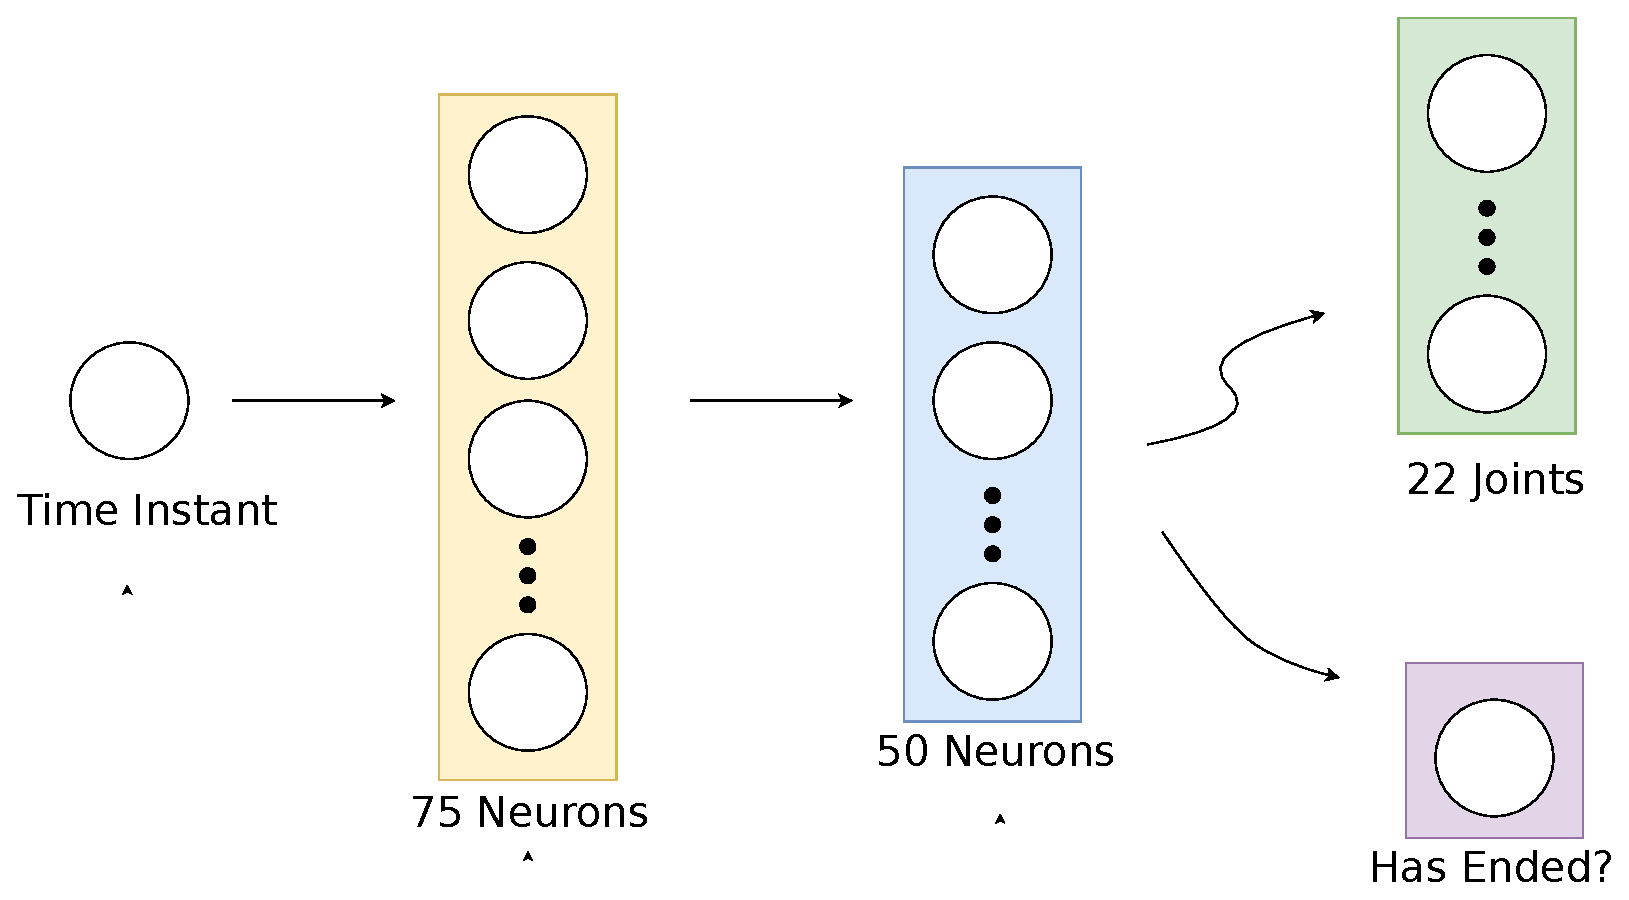
\includegraphics[width=0.5\textwidth]{Cap5/architecture}
\caption{The architecture of a neural network designed to learn motions.}
\label{fig:model_plot}
\end{figure}

This architecture resulted in thousand of parameters to optimize, as exposed in Table \ref{tab:network_summary}. A very high number, when compared to more traditional optimization approaches \cite{AAAI12-MacAlpine}. Notice that, by increasing the number of parameters usually allows representing better movements.

\begin{table}[htbp]
\caption{The Network Summary}
\begin{center}
\begin{tabular}{|c|c|c|c|}
\hline
\textbf{Layer}&{\textbf{Neurons}}& \textbf{Activation}& \textbf{Parameters} \\
\hline
Dense & 75 & LeakyReLU & 130  \\
\hline
Dense & 50 & LeakyReLU & 3800 \\
\hline
Dense & 23 & Linear & 1173 \\
\hline
\end{tabular}
\begin{tabular}{|c|c|}
\hline
\textbf{Total Parameters} & 5123 \\
\hline
\end{tabular}
\label{tab:network_summary}
\end{center}
\end{table}


\section{The Training Procedure}
Since keyframe motions are executed in an open-loop fashion, the sequence of joint positions are always the same for different repetitions, independently of robot's state. Therefore, by adding samples of multiple executions of the same motion would not make our dataset richer. So, we decided to use only one repetition for each movement for faster training. In the case of the walking motion, we collected samples within one walking period.

During the training, we used 50 thousands epochs divided into 5 training phases, where the learning rate was decreased between phases, in order to achieve better performance. First, we executed 30000 epochs, by using the learning rate of 0.001. The other phases had 5000 epochs each, and we decreased the learning rate by 0.0002 in each phase.

Furthermore, we used Adam optimization \cite{adam2014}, during the whole training. The loss function used was the mean squared error, as explained in Subsec. \ref{sec:neural_networks}. We decided this loss function is adequate for this problem, mainly because it strongly penalizes large errors, which can collapse the whole motion.

\section{The Deployment in the Soccer 3D Environment}
In order to perform the network design and the training procedure, we used the Keras \cite{chollet2015keras} framework coupled with Tensorflow \cite{tensorflow2015-whitepaper} as backend. After training, the weights were frozen and converted to a specific format, which was readable, by using the Tensorflow C++ API integrated within agent's code. Hence, the training was performed outside the environment, but the agent actually has computed network inferences, during the simulation execution.
